% Chapter 1

\chapter{Introduction} % Main chapter title

\label{Chapter1} % For referencing the chapter elsewhere, use \ref{Chapter1} 

%----------------------------------------------------------------------------------------

% Define some commands to keep the formatting separated from the content 
\newcommand{\keyword}[1]{\textbf{#1}}
\newcommand{\tabhead}[1]{\textbf{#1}}
\newcommand{\code}[1]{\texttt{#1}}
\newcommand{\file}[1]{\texttt{\bfseries#1}}
\newcommand{\option}[1]{\texttt{\itshape#1}}

%-------------------------------------------------------------------------------------


In an age where there is an exponentially increasing volume of data being produced, the ability for a user to get the information they seek has become ever more challenging \cite{sintef2013bigdata}. The abundance of information which gives an overwhelming number of options to a user when making a decision is known as the information overload problem \cite{bawden2020information}. With the vast amount of information available, it can be challenging for users to find items or products that meet their preferences or needs. Recommender systems are tools which directly aim to address the challenge of information overload \cite{o2005trust}. The general idea behind a recommender system is to narrow down the perceived available options and present a limited set of personalised choices (recommendations) based on said user’s preferences, behaviour and or other relevant factors \cite{o2005trust}. In this light, a recommender system can be seen as a filtration tool which greatly washes out undesirable results and brings forth content desired or more relevant to a user’s current interests and needs. In this way they are able to help to reduce information overload and make the decision-making process easier and more efficient. A lucrative byproduct of this is an improved overall user experience, increased engagement and user satisfaction. Given these outcomes, recommender systems have become a highly researched area over recent years \cite{seth2022comparative}. Recommender systems are a crucial tool in the arsenal of e-commerce platforms which try to help consumers navigate through an abundance of product options. To this end, recommender systems are capable of enhancing the customer experience by showing products that they are inclined to want and thus also boost sales of these product. The apparent effectiveness of these systems has led to this surge in research in this domain. In this thesis, we aim to directly contribute to this area of research by developing and extending upon an established recommender system method by incorporating data from multiple modalities and investigates the potential impact of incorporating this additional modality in improving the accuracy of recommendations. 

This chapter will introduce recommender systems in Section \ref{sec:1 Recommender Systems: definition and types} along with the different recommender paradigms which have gained a lot of attention in this study area. In Section \ref{sec:1 Research Problem and Objectives} we draw light to the research problem and objectives of this paper. The specific research questions and significance of this paper is explained in Section \ref{sec:1 Research Questions and Significance} in detail before concluding the chapter by explaining the structure of the remaining sections of this paper in Section \ref{sec:Dissertation Outline}.


%-------------------------------------------------------------------------------------
\section{Recommender Systems: definition and types}
\label{sec:1 Recommender Systems: definition and types}
A recommender system is a type of information filtering system that seeks to predict user preferences or interests by generating \textit{recommended} items such as products, services or content that the user is likely to be interested in \cite{seth2022comparative}. “Item” is the general term used to denote what the system recommends. Instead of sifting through irrelevant information and products, users are presented with content and products that are more likely to be of interest to them. Recommender systems have quickly become a necessity, given that users cannot search through an abundance of content to connect with products, services or knowledge (i.e., items) that are important to them \cite{seth2022comparative}. 

Recommender systems deal with two types of information: characteristic information, which includes details about the items, such as keywords or categories; and user-item interactions, which encompass data like user ratings or likes and so on.  With respect to the types of recommender systems available, the data (ratings data, item characteristics data, etc.) also plays an important role in determining which recommender system would be effective. In the field of recommender systems, there exist three main branches: collaborative filtering, content-based filtering and hybrid systems \cite{thorat2015survey}.

\textbf{Collaborative-based filtering}, probably the most extensively implemented type of recommender, is based based on historical user-item interactions \cite{thorat2015survey}. It operates by analysing patterns of user preferences across items to make predictions or suggestions. The collaborative filtering methods do not rely on explicit domain knowledge or item attributes but rather on the collective wisdom embedded within the data. At a high level, there are two types of collaborative filtering algorithms which have been proposed in the literature: memory-based algorithms, which rely on computing the similarity between users or items in order to make recommendations, and model-based algorithms, which rely on building a model or mathematical representation of the data to make recommendations \cite{thorat2015survey}. Both memory-based and model-based algorithms have their strengths and weaknesses which we discuss further later on. 

\textbf{Content-based filtering}, by contrast, is based on characteristic information and works by understanding the underlying features (or characteristics) of each item \cite{thorat2015survey}. There is no general high-level categories for which content-based filtering algorithms are universally recognised, as like we have for collaborative-based filtering (model-based vs memory-based). Regardless, the idea is that a content-based filtering algorithm analyses the features of an item and then recommends other items with similar features. These features could be the attributes of an item, like the colour or style of a product, or they could be keywords, like the genres or artist names of a song. 

We often find in practice that these two types of recommender system techniques (collaborative and content-based) are combined to form \textbf{hybrid systems} \cite{thorat2015survey}. These use both types of information, with the idea to leverage the strengths of each individual method to improve the accuracy and relevance of the recommendations, whilst also avoiding problems that are generated when working with just one kind of system \cite{thorat2015survey}. These hybrid modelling approaches have been shown to outperform individual algorithms in many cases, however they also carry with it additional complexities in terms of model building and efficiency \cite{ccano2017hybrid}. Furthermore, whilst combining different models can often produce a more accurate model, there are other approaches that can be used to improve the accuracy and relevance of recommendations. One such approach is using multi-modal recommender systems, which leverage multiple types of data or information sources to make recommendations \cite{ccano2017hybrid}. Figure \ref{fig:types_recommenders} shows at a high-level, the main types of recommender systems and the popular subcategories within these branches. Note that hybrid recommenders, like content-based filtering, do not necessarily have recognised high-level categories, however some approaches can be bundled into some high-level categories such as weighted approaches.

\begin{figure}[h]
    \centering
    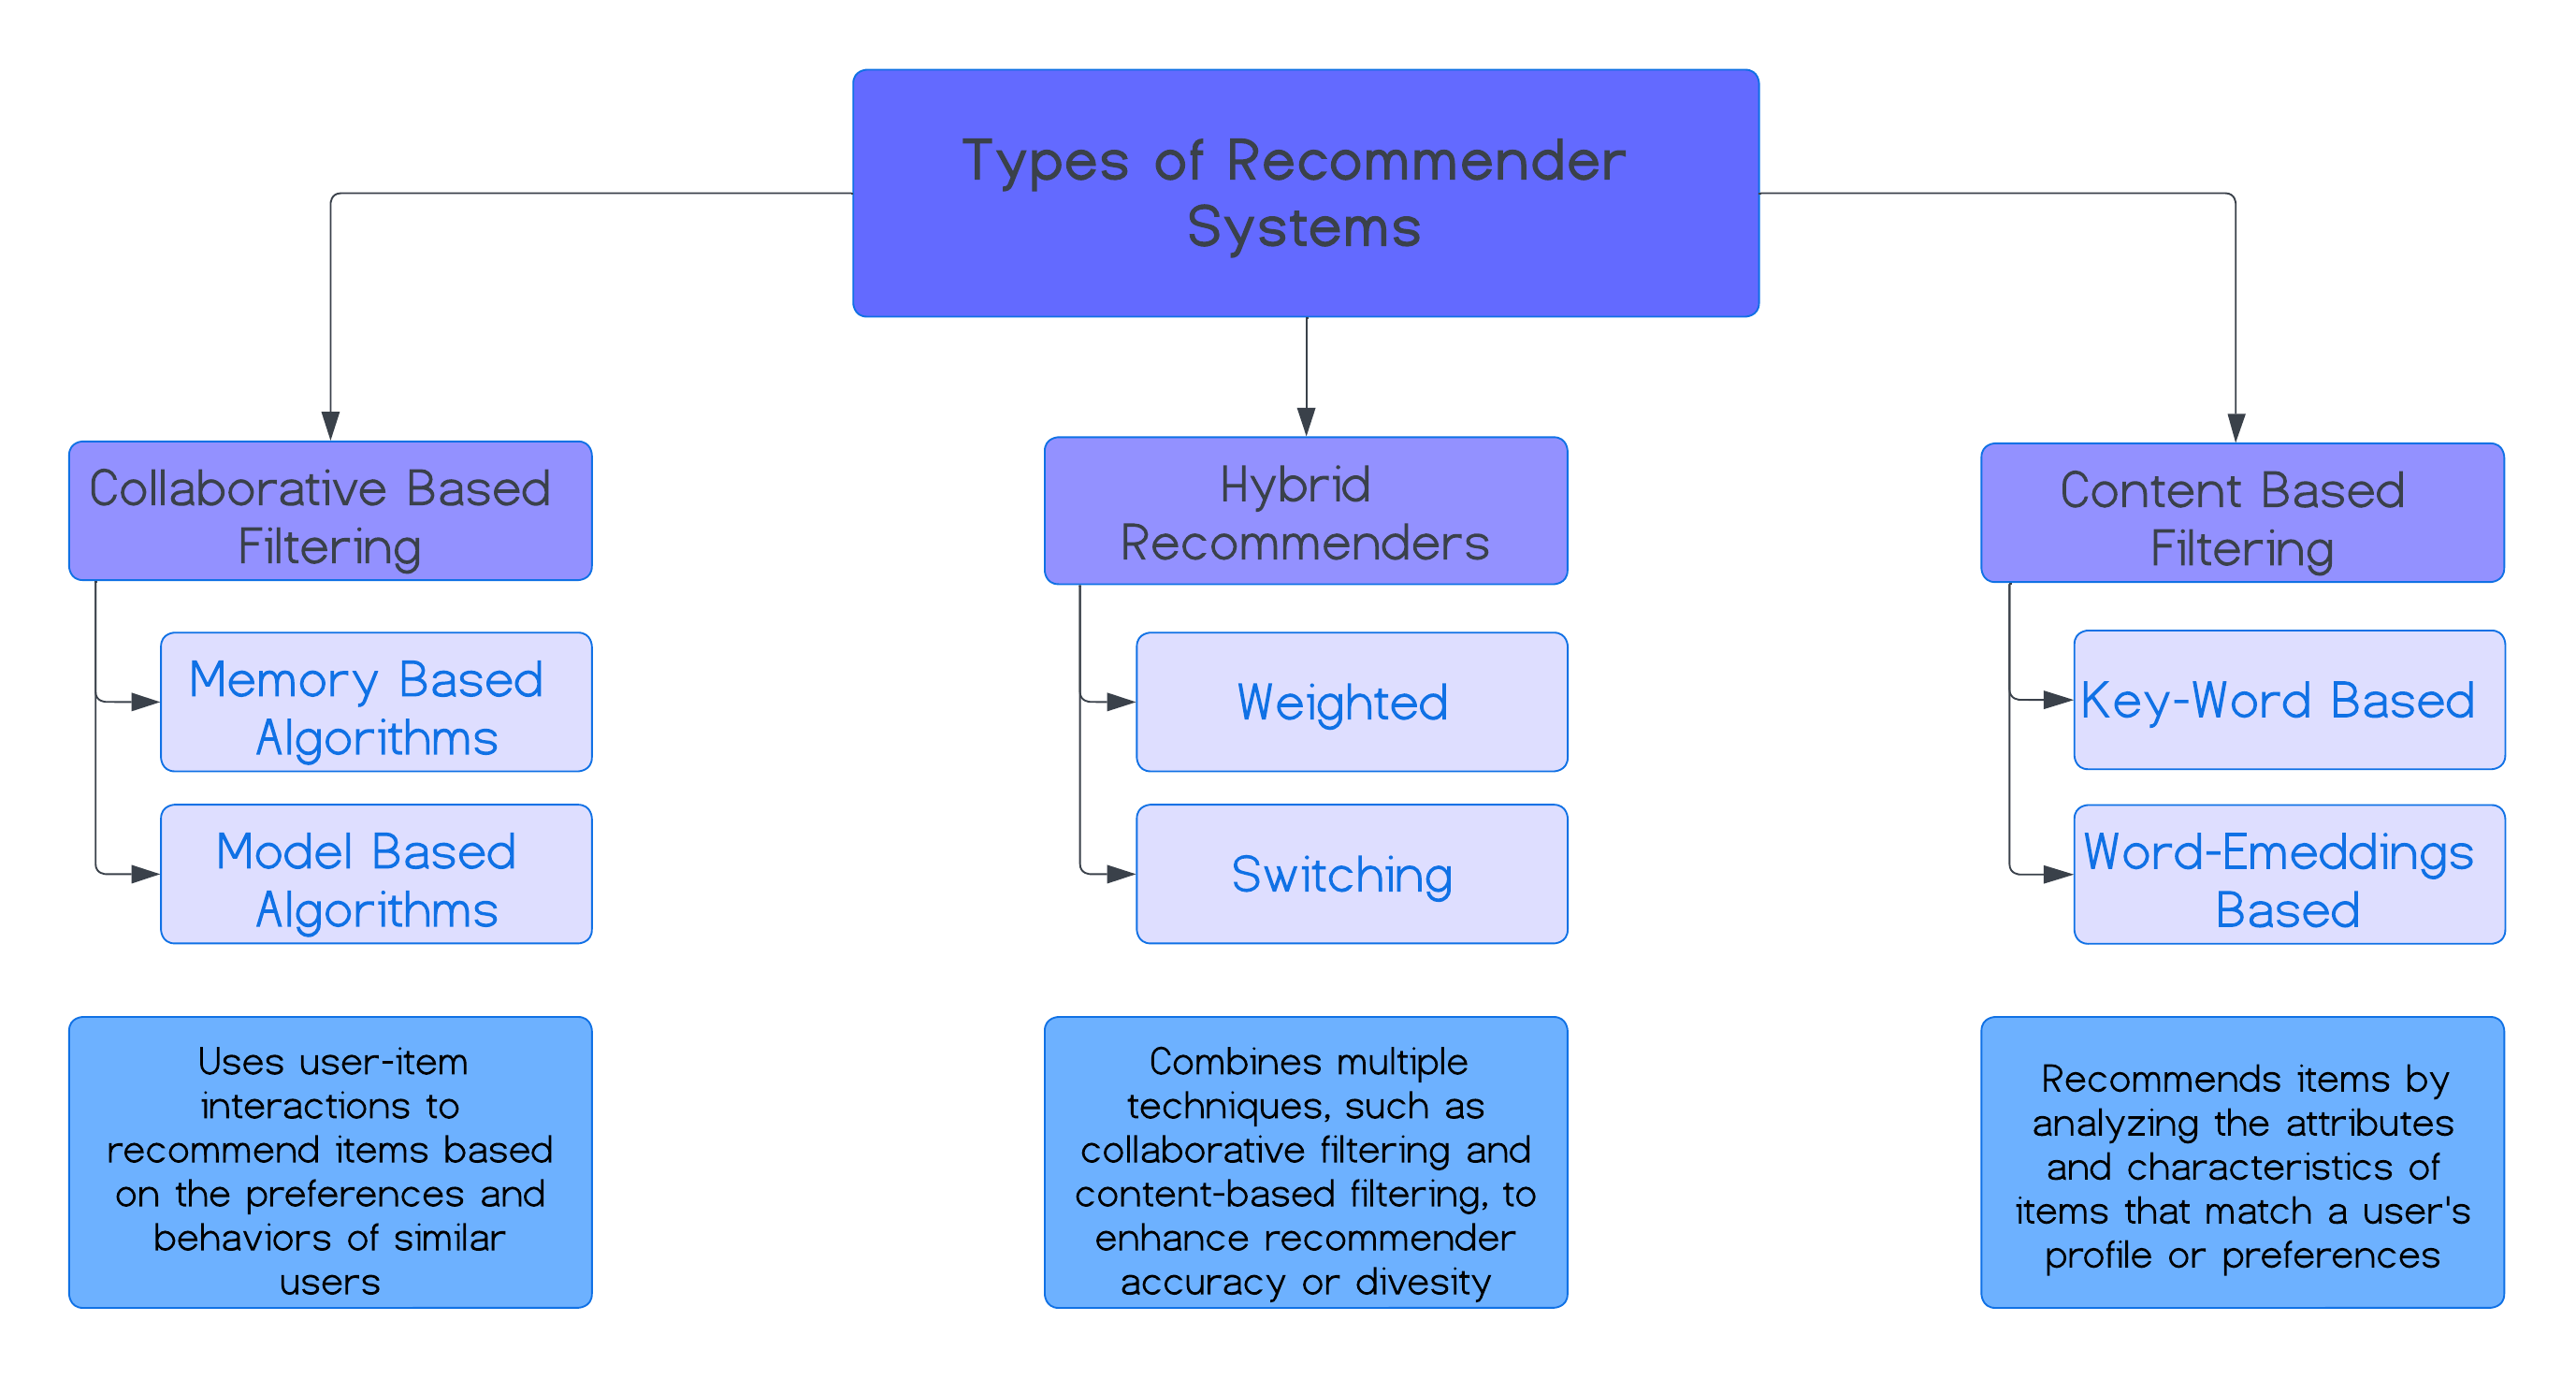
\includegraphics[width=0.9\textwidth]{Figures/Untitled.png} % Adjust the width as needed
    \caption{The different types of recommender systems.}
    \label{fig:types_recommenders}
  \end{figure}
  
Multi-modal refers to the integration of different types or modes of data in a system \cite{truong2021multi}. In the context of recommender systems, multi-modal simply refers to the use of multiple types of data to make recommendations. By combining information from different modalities, such as text, images, audio, and video, multi-modal recommender systems can provide a more comprehensive understanding of user preferences and offer more personalised recommendations \cite{truong2021multi}. Using multi-modalities also poses the opportunity to alleviate data sparsity\footnote{the situation where the available data is highly incomplete, resulting in numerous missing values in the user-item interactions. This occurs due to the vast number of items and limited user interactions, making accurate predictions for less observed items challenging} by leveraging or including auxiliary information that may encode additional clues on how users consume items. Examples of such data (referred to as modalities) are social networks, item’s descriptive text, or customer product reviews \cite{truong2021multi}. Studies on multi-modal recommender systems have become a popular topic in the field as many understand the potential upside of incorporating multiple data types into a prediction algorithm \cite{truong2021multi}. In fact, multi-modal recommendation systems have become the industry standard and are widely used across many domains as companies try to personalise their products and services to better meet the needs and preferences of their customers \cite{liu2023multimodal}. For example, in e-commerce, a multi-modal recommender system can take advantage of product images and descriptions, user reviews, and purchase history to make recommendations \cite{liu2023multimodal}. Beyond multi-modalities, recommender systems have evolved to incorporate deep learning technologies. Traditional recommender systems have shown to be effective in many cases, however the recent advances in deep learning over the past decade have opened up new opportunities for improving the accuracy and personalisation of recommendations. 

Deep learning is a a subset of machine learning that deals with models that are comprised of multiple layers (hence the “deep” in deep learning). In the context of recommender systems, deep learning algorithms can be used to effectively extract complex patterns and relationships from large amounts of data \cite{he2017neural}. This is particularly attractive since the goal is to predict user preferences based on past behaviours or interactions. We shall explore the application of deep learning in the context of our recommender system by employing a neural collaborative framework which essentially generalises and puts forth a neural network based approach to matrix factorisation (which is extensively used in collaborative filtering) to improve the accuracy of rating predictions \cite{he2017neural}. Amazon, amongst many other internet giants, also use neural networks in their recommendation engine to make product recommendations \cite{steck2021deep}. 

Although these systems can easily be mistaken as simply a tool for information retrieval and data discovery - in industry their importance is unwavering \cite{he2017neural}. With the tremendous amount of data available online, recommender systems are held in high regard amongst large internet corporations, research and investment \cite{steck2021deep}. 

\section{Research Problem and Objectives}
\label{sec:1 Research Problem and Objectives}

The aim of this thesis is to directly enhance the predictive accuracy of recommender systems by developing a neural collaborative filtering (NCF) model that incorporates data from multiple modalities (types), exploiting explicit numeric product ratings and product review text data as well user review sentiments. The idea is that by using this auxiliary information we can aid the NCF system account for the nuances and complexities of user preferences that may be expressed through textual data. We build on the existing work done by \cite{he2017neural} on NCF systems and several other works (\cite{srifi2020recommender}; \cite{zhang2014urcf}) which laid the groundwork to effectively incorporate auxiliary information into collaborative filtering systems (including user reviews). As such, this thesis seeks to investigate the potential of incorporating product review text and review text sentiment as additional sources of information to improve the predictive accuracy of recommendations. 

This is achieved by building a NCF recommender system which processes the explicit ratings data and is also augmented with textual features (product reviews) and sentiments (review sentiments) to form a multi-modal system. Building this neural network architecture (for collaborative filtering) enables the system to learn a non-linear mapping between the input features (i.e., item attributes) and the target output (i.e., user preferences) \cite{he2017neural}. Through comparative evaluation with benchmark recommender models, the efficacy of the proposed multi-modal recommender will be assessed, with a particular focus on its ability to provide predict accurate ratings for unseen items. To this end, a number of different models will be trained, evaluated and compared to one another in an effort to establish the performance benefits of different models. The research questions presented in Section \ref{sec:1 Research Questions and Significance} will guide this process.

Ultimately, this thesis aims to contribute to the development of a more effective and efficient recommender system that can potentially leverage the additional textual information provided by users for products which can potentially aid in generating recommendations tailored to the unique preferences and needs of individual users.

\section{Research Questions and Significance}
\label{sec:1 Research Questions and Significance}

As mentioned, this paper seeks to explore the impact of incorporating product reviews and review sentiments into a recommender system model whilst also evaluating the performance of the NCF model. Recommender systems have become pivotal to the way companies interact and sell their products to their consumers \cite{steck2021deep}. A recommender system’s ability to accurately predict consumer interests and desires on a highly personalised level make them a very valuable tool for content and product providers, like Amazon, Google amongst other technology giants. The key research questions addressed in this paper are discussed and explained below. 





\begin{enumerate}
    \item \textbf{How does incorporating product reviews into a recommender system model impact the accuracy of the system’s recommendations?} 
    
    Here we are interested in determining whether integrating user reviews into a recommendation algorithm leads to more accurate and relevant product suggestions for users. Another way of looking at this is examining the accuracy of a multi-modal recommender system compared to that of a single-modal recommender system - i.e., a recommender that relies on only one type of data. User reviews for products could potentially provide additional insights into user preferences or product features that are not captured by the metadata. However, reviews may also introduce noise or biases into the recommendation algorithm which can lead to less accurate suggestions \cite{zhang2014urcf}. Findings from this study could provide further scope for incorporating review text into product recommendation designs or highlight potential pitfalls to avoid when integrating user reviews. The study also may prove to provide further support for multi-modal recommender systems. 


    \item \textbf{How does incorporating review sentiment as well as review text in a recommender system impact the accuracy of the system's recommendations?} 
    
    Incorporating sentiment analysis into a recommender system introduces an avenue for the integration of additional features that can contribute to enhancing recommendation accuracy. Sentiment analysis, as a technique to assess the emotional tone and polarity of textual content such as product reviews, offers a means of extracting valuable insights from user-generated content \cite{medhat2014sentiment}. By incorporating sentiment analysis outcomes alongside traditional recommendation factors, the system gains access to a richer set of attributes that can potentially capture nuanced user preferences and sentiments. 

    The impact of sentiment analysis on accuracy of recommender systems provides scope to further utilise review text in possibly improving recommendation accuracy. Potential findings from this study could provide insights into the most effective sentiment analysis techniques for collaborative-based recommender systems and inform the design of more accurate and effective recommendation algorithms. Conversely, the study could highlight potential challenges and limitations of using sentiment analysis in a recommender system, such as accuracy issues due to sarcasm, ambiguity, or variations in language use. 

    \item \textbf{How does the performance of the collaborative-based filtering recommender system using neural collaborative filtering compare to that of popular benchmark collaborative-based recommender systems?} 
    
    The general idea is that incorporating deep learning into a collaborative filtering model can alleviate the fragility of simpler more traditional collaborative-based filtering models in capturing user preference profiles, and as such improve accuracy of recommendations. This is another key area of interest in our study - examining the potential capacity of neural collaborative filtering system to outperform other popular collaborative-based recommender systems. In evaluating our recommender system, we assess its predictive accuracy (as well as its top-n generation) against other benchmark models. The architecture and technical details of all the developed models are provided in detail in Chapter \ref{Chapter4} - the methodology.  Deep learning models are by design more complex and often have greater computational expense and slower processing than more traditional models under collaborative filtering \cite{he2017neural}. By investigating the potential advantage these deep learning systems have could highlight the potential trade-off between the level of desired complexity and performance. Whilst this will be domain specific and depend on the needs and resources available, the study will contribute to providing additional insight into this field. 
    
    \item \textbf{What are the potential trade-offs of incorporating product reviews into a recommender system, such as increased complexity or potential biases in the recommendations?} 
    
    Product reviews can often contain large amounts of unstructured data which is cause for concern for recommender systems, which need to quickly process and integrate this information in their algorithm. Another potential concern may be the bias inherent in user reviews. These will be discussed in depth later on in this paper. However, findings from this study could prove to be useful in highlighting the potential benefits and drawbacks of incorporating product reviews into a recommender system. Furthermore, it could open up paths for discussion on potential strategies for mitigating the trade-offs of using reviews in recommendation algorithms, such as developing more sophisticated sentiment analysis techniques. 
\end{enumerate}

    
These key research questions will be referenced greatly throughout the whole paper. The significance of the findings from the study ultimately provides further support for possible future design and implementations in this space. More specifically, findings will directly contribute to the existing literature on recommender systems and provide insights into the effectiveness and limitations of incorporating product reviews and sentiment analysis features in collaborative models, as well as the trade-offs associated with these approaches.

% %-------------------------------------------------------------
\section{Dissertation Outline}
\label{sec:Dissertation Outline}

In this chapter we introduced what recommender systems are and the importance of them as tools to help users find the content and services they seek (or may want). Specifically, recommenders alleviate the information overload problem directly and enable users to find information as well as discover items that align to their preferences. We have also described the aim of this thesis, and the research questions it will seek to answer in \ref{sec:1 Research Questions and Significance}. It has also introduced the primary collaborative-based multi-modal recommender system which we will be developing and examining in this thesis - NCF. 

Chapter 2 is a detailed literature review which provides context for this research by first addressing the history and application of recommender systems in E-commerce. This history will start with a brief exploration of the fundamental concepts in recommender systems which have remained relevant since their inception in Section \ref{sec:2 Recommender Systems: history and applications}. We shall also describe the immediate benefit and advantage that recommender systems have provided for the E-commerce industry. From here, in Section \ref{sec:2 Collaborative Filtering}, we shall explore the main recommender system paradigm of concern for this paper: collaborative filtering. Here, a brief history of the algorithms are discussed as well as the latest breakthroughs. This will lead into a discussion on the deep learning era in Section \ref{sec:2 Deep Learning in Recommender Systems}, where recent advances are of particular importance. Additionally, we explore the prevalence of text and its applications for recommender systems in \ref{sec:2 Text Analysis in Recommender Systems}, other types of recommenders in section \ref{sec:2 Other Recommenders: a brief overview and history} and finally the key evaluation methods used in recommender system research in Section \ref{sec:2 Evaluation Methods}. The chapter closes with addressing the various limitations and challenges faced by collaborative filtering and recommender systems as a whole. Chapter \ref{Chapter3} addresses all matters relating to data. In order to critically examine our NCF recommender system and assess impacts of additional features, it is necessary to have a source of user-item data. Our source is the Amazon Product Review dataset, which is publicly available and is discussed in further detail in Section \ref{subsec:3 Amazon Review Dataset}. In addition to describing (\ref{sec:Variable Description}) and explaining the variables and the data collection process (\ref{sec:3 Data Collection and Preprocessing}), we explore the dataset in Section \ref{sec:3 Trends and Patterns}. Finally, we summarise our findings and partitioning process, in Sections \ref{subsec:3 Data Summary} and \ref{sec:3 Data Partitioning} respectively. Chapter \ref{Chapter4} looks at the methods used in our research. It provides all the technical details necessary to understand the models utilised and trained. We begin the Chapter by detailing out our overall modelling approach in Section \ref{sec:4 Modelling Approach} before diving into the details. The groundwork for this will be built in Section \ref{sec:4 Neural Collaborative Filtering}, where the basic architecture and training procedure for neural collaborative filtering will be discussed in length. Additionally, Section \ref{sec:4 Benchmark Models} discusses the various benchmark models that shall be built to assess the performance of the neural collaborative model. Finally, Section \ref{sec:4 Evaluation} details the evaluation criteria that shall be employed to assess our recommender models. Chapter \ref{Chapter5} documents the observed results (Section \ref{sec:5 Results}) as well as a detailed discussion of them (Section \ref{sec:5 Discussion}) with frequent reference to the research questions raised from this Chapter (\ref{Chapter1}).  Chapter \ref{Chapter6} will summarise (\ref{sec:6 Summary of Results and Findings}), expand on limitations (sec:6 Limitations) and further work (\ref{sec:6 Future Work}), as well as conclude this paper (\ref{sec:6 Conclusion}). 






